\documentclass[12pt]{report}
\usepackage{lipsum}
\usepackage{mathtools}
\usepackage{array}
\usepackage{colortbl}
\usepackage{chemfig}
\RequirePackage[left=3cm,top=1.5cm,right=3cm,bottom=2.5cm,nohead,nofoot]{geometry}

\begin{document}

\thispagestyle{empty}   % this page does not have a header

\tableofcontents

\chapter{Introduction}

\chapter{Output Summary}

\chapter{Background Research}


\section{What is computer vision?}


Computer vision (CV) is a scientific discipline that studies how computer scan efficiently perceive, process, and understand information from visual data such as images and videos.

As humans, we can classify three-dimensional objects with ease, whether the pictures are the same object with different colours or angles, we are good at determining the object we are classifying. 
Computer vision has been developed to detect edges from a pixelated image, face detection, and has been used to develop 3D models from a snapshot yet the technology we have today could be compared to a young child's biological vision. 

Computer vision is used in various real world application such as traffic surveillance or medical imaging (SZELISKI, 2020), where people are now able to utilize magnetic resonance imaging (MRI) to safely analysis the heart wall motion where the end result is a 3d model of the heart pumping (Metaxas, 1997). 

In recent years, computer vision has been adapting deep learning algorithms to efficiently classify unseen objects within pixel images and videos. 


\section{Deep learning}

Deep learning uses artificial intelligence (AI) to try and simulate the choices that a human brain will make. Problems that have regression or classification outputs can be solved by passing data/inputs through artificial neurons which were previously tweaked for the specific problem by training data. There are many different variants of deep learning algorithms such as Artificial Neural Networks (ANN) or Long Short-Term Memory (LSTM) Networks (Hochreiter, 1997) which build onto each other.

\subsection{Neural networks (NN)}

Neural networks is a network formed of interconnected perceptrons which each carry weights and biases. The weights (w) and biases (b) are each represented by a float value which are used to multiply and add to the input respectively. The outcome is then put into an activation function (e.g. ReLU or sigmoid) which determines if the neuron should be activated. These activations chain together to output a value of what the neural network thinks the solution is. 

\vspace{5 mm}

\begin{centering}
	
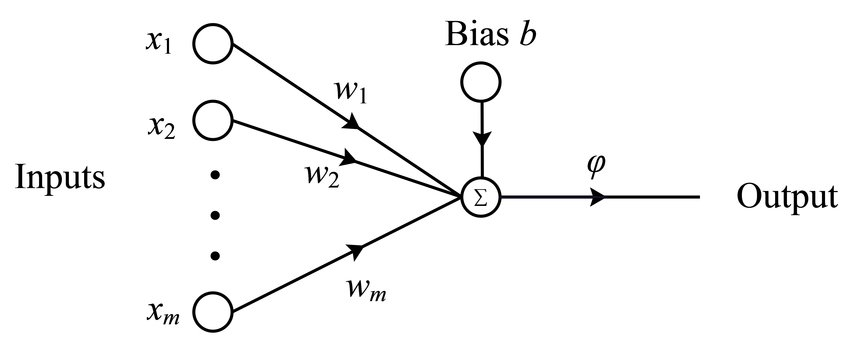
\includegraphics[width=100mm]{./images/weights and biases.png}

{Figure 1: A single perceptron with inputs, weights, and biases}

\end{centering}

\vspace{5 mm}

The values of weights and biases are updated when training data is pass through the network using back propagation, adjusting their values depending on the actual and network's solution to the problem. A network can have multiple layers of several perceptrons in order to solve more complex problems, but has the down side of overfitting the accuracy of the output.


\subsection{Convolutional neural networks (CNN)}

CNNs builds upon the NN, specialising in working with grid-structured data such as images or videos. Unlike NN which takes in a 1 dimensional vector as its input, CNN uses tensors (high dimensional vector/matrix) for processing images. The convolutional layer of the network includes kernels/filters (a type of matrix) which efficiently detects features within an image by calculate the sum of the kernel multiplied by a subgrid of the image. These filters are trained to extract details within the images, and to make better predictions over the course of training. Different techniques can be applied such padding to reduce the lost of data when filtering.

The information about the deep learning architectures we have discussed were influenced by taking part in the 'Introduction to AI' (IN3062) and 'Programming and Mathematics for Artificial Intelligence' (IN3063) module at City University.

\section{WILDTRACK dataset}

The 'WILDTRACK' dataset provides footage of pedestrians from 7 different angle, each video having a length of 60 minutes and were filmed using three 'GoPro Hero 4' and four 'GoPro Hero 3' at high resolution (1920x1080). The location of the video took place near a public research university called ETH Zurich, Switzerland. The cameras used were calibrated to allow for precise calculations when wanting the distance between two objects.

While there are other datasets that offer similar features such as the 'EPFL-RLC' dataset, the videos themselves do not contain the same density of pedestrians relative to the 'WILDTRACK' dataset.Footage from other datasets showcase people who are more static, making it less challenging for the project.

\subsection{Research papers with WILDTRACK dataset}

There are many published research papers that have used this dataset for their own project. For example, a research paper that was dedicated to detecting the same pedestrian using all camera footage and creating a shared top down view of the 'point of interest' which indicates the location of the pedestrians (López-Cifuentes A. 2018). What was interesting about this paper was that the author used another dataset that did not include calibrated cameras. When comparing the results at the end, the accuracy of the 'WILDTRACK' was marginally better as the other dataset had calibration errors, therefore the 'point of interest' were at different locations when looking at the shared top down view.


\section{Existing systems}

Many different social distancing detections have been made ever since the outbreak of the corona virus. Most of the systems use deep learning architectures paired with the OpenCV library to help classify pedestrians within a video.

\subsection{Example (Y. C. Hou, 2020)}

This system uses a combination of the YOLO (You Only Look Once) model with the COCO (Common Objects in Context) dataset to train their model. The goal of the project was to produce a top down view of the pedestrians, showing the distance between each person who were identified within the frame. The results of the system were very accurate, as they were able to make use of calibrated cameras. What was very interesting about the project is that some pedestrians were not classified due to hiding behind others. This showcases the limitation of the dataset used, as there were no overlapping footage of the field of view. Further improvements to the system were suggested such as mask and human body temperature detection. The system overall is similar to what this project will achieve with the difference of dataset.


\end{document}